\index{function regression}
\index{pattern recognition}
\index{optimal control}
\index{inverse problems}
\index{optimal shape design}
\index{function optimization}

Learning tasks for neural networks can be classified according to the source of information for them. 
There are basically two sources of information: data sets and mathematical models. 
In this way, some classes of learning tasks which learn from data sets are function regression, pattern recognition or time series prediction. 
On the other hand, learning tasks in which learning is performed from mathematical models are optimal control or optimal shape design. 
Finally, in inverse problems the neural network learns from both data sets and mathematical models.

\subsubsection*{Function regression}

Function regression is the most popular learning task for neural networks. 
It is also called modelling. The function regression problem can be regarded as the problem of
approximating a function from a data set consisting of input-target instances
\cite{Haykin1994}. The targets are a specification
of what the response to the inputs should be \cite{Bishop1995}. 
While input variables might be quantitative or qualitative, in function regression target variables are quantitative. 

Performance measures for function regression are based on a sum of errors between the outputs from the neural network and the targets in the training data. 
As the training data is usually defficient, a regularization term might be required in order to solve the problem correctly.  

An example is to design an instrument that can determine serum cholesterol levels from
measurements of spectral content of a blood sample. There are a number of 
patients for which there are measurements of several wavelengths of the spectrum.
For the same patients there are also measurements of several
cholesterol levels, based on serum separation \cite{Demuth2009}. 

\subsubsection*{Pattern recognition}

The learning task of pattern recognition gives raise to artificial intelligence. That problem can be stated as
the process whereby a received pattern, characterized by a distinct
set of features, is assigned to one of a prescribed number of
classes \cite{Haykin1994}. Pattern recognition is also known as classification. Here
the neural network learns from knowledge represented by a training
data set consisting of input-target instances. The inputs include a
set of features which characterize a pattern, and they can be quantitative or qualitative. The targets specify
the class that each pattern belongs to and therefore are qualitative \cite{Bishop1995}.

Classification problems can be, in fact, formulated as being modelling problems. 
As a consequence, performance functionals used here are also based on the sum squared error. 
Anyway, the learning task of pattern recognition is more difficult to solve than that of function regression. 
This means that a good knowledge of the state of the technique is recommended for success. 

A typical example is to disinguish hand-written versions of characters. 
Images of the characters might be captured and fed to a computer. 
An algorithm is then seek to which can distinguish as reliably as possible between the characters \cite{Bishop1995}. 

\subsubsection*{Optimal control}

Optimal control is playing an increasingly important role in the
design of modern engineering systems. The aim
here is the optimization, in some defined sense, of a physical
process. More specifically, the objective of these problems is to
determine the control signals that will cause a process to satisfy
the physical constraints and at the same time minimize or maximize
some performance criterion \cite{Kirk1970} \cite{BalsaCanto2001}. 

The knowledge in optimal control problems is not represented in the form of a data set, it is given by a mathematical model. 
These objective functionals are often defined by integrals, ordinary differential equations or partial differential equations. 
In this way, and in order to evaluate them, we might need to apply Simpon methods, Runge-Kutta methods or finite element methods. 
Optimal control problems often include constraints. 

As a simple example, consider the problem of a rocket launching a
satellite into an orbit around the earth. An associated optimal
control problem is to choose the controls (the thrust attitude angle
and the rate of emission of the exhaust gases) so that the rocket
takes the satellite into its prescribed orbit with minimum
expenditure of fuel or in minimum time.

\subsubsection*{Optimal shape design}

Optimal shape design is a very interesting field for industrial
applications. The goal in these problems
is to computerize the development process of some tool, and
therefore shorten the time it takes to create or to improve the
existing one. Being more precise, in an optimal shape design process
one wishes to optimize some performance criterium involving the
solution of a mathematical model with respect to its domain of
definition \cite{Bucur2005}. 

As in the previous case, the neural network here learns from a mathematical model. 
Evaluation of the performance functional here might also need the integration of functions, ordinary differential equations or partial differential equations. 
Optimal shape design problems defined by partial differential equations are challenging applications. 

One example is the design of airfoils,
which proceeds from a knowledge of computational fluid dynamics
\cite{Eyi1994} \cite{Mohammadi2004}. The performance goal here might
vary, but increasing lift and reducing drag are among the most common. Other objectives as weight reduction, stress reinforcement and
even noise reduction can be obtained. On the other hand, the airfoil
may be required to achieve this performance with constraints on
thickness, pitching moment, etc.

\subsubsection*{Inverse problems}

Inverse problems can be described as being opposed to direct
problems. In a direct problem the cause is given, and the effect is
determined. In an inverse problem the effect is given, and the cause
is estimated \cite{Kirsch1996} \cite{Sabatier2000} \cite{Ramm2005}.
There are two main types of inverse problems: input estimation, in
which the system properties and output are known and the input is to
be estimated; and properties estimation, in which the the system
input and output are known and the properties are to be estimated.
Inverse problems can be found in many areas of science and
engineering. 

This type of problems is of great interest from both a theoretical and practical perspectives. 
From a theoretical point of view, the neural network here needs both mathematical models and data sets. 
The aim is usually formulated as to find properties or inputs which make a mathematical model to comply with the data set. 
From a practical point of view, most numerical software must be tuned up before being on production. 
That means that the particular properties of a system must be properly estimated in order to simulate it well.

A typical inverse problem in geophysics is to find the 
subsurface inhomogeneities from collected scattered fields caused by
acoustic waves sent at the surface and a mathematical model of soil mechanics.  

\subsubsection*{Tasks companion diagram}

As we have said, the knowledge for a neural network can be represented in the form of data sets or mathematical models. 
The neural network learns from data sets in function regression and pattern recognition; 
it learns from mathematical models in optimal control and optimal shape design; 
and it learns from both mathematical models and data sets in inverse problems. 
Please note that other possible applications can be added to these learning tasks. 

Figure \ref{LearningTasksFigure} shows the learning tasks for neural networks described in this section. 
As we can see, they are capable of dealing with a great range of applications. 
Any of that learning tasks is formulated as being a variational problem. 
All of them are solved using the three step approach described in the previous section. 
Modelling and classification are the most traditional; 
optimal control, optimal shape design and inverse problems can also be very useful. 

\begin{figure}[h!]
\begin{center}
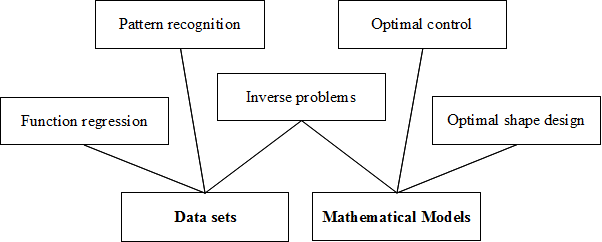
\includegraphics[width=1.0\textwidth]{neural_networks_basis/learning_tasks}
\caption{Learning tasks for neural networks.}\label{LearningTasksFigure}
\end{center}
\end{figure}
